% Deadline contracts: results. Every number is taken from the saved study outputs:
% data/research/pm_hazard/summary.json (keys noted next to each table and key number).

\subsubsection{Implied hazards are too high, most of all in the last day}\label{haz-res-calib}

\Cref{haz-tab-calib} reports the hazard multiplier $k$ of \cref{haz-eq-k} for the pooled event,
mention and count contracts, by lead and split. In the \estim{} the implied hazard is too high at
every lead. Realised hazards are about 61\% of implied ones within a day of the deadline and 61--79\%
at longer leads, and every 90\% interval lies below one. In cents, prices exceed realised frequencies
by 1.2--8.6\cents{} per contract, and the gap grows with the lead because longer windows carry
higher prices. The holdout confirms the near-deadline result: $k=0.62$ within six hours and $0.51$ at
6--24 hours, with intervals below one. Beyond three days the holdout point estimates lie between 0.69
and 0.98, but with 23--52 clusters per cell the intervals include one.
% source: summary.json:calibration_by_split (group core)

\begin{table}[t]
\centering
\begin{threeparttable}
\caption{Calibration of implied hazards by lead (events, mentions and counts)}\label{haz-tab-calib}
\footnotesize
% source: data/research/pm_hazard/summary.json:calibration_by_split (group = core)
\setlength{\tabcolsep}{3.5pt}
\begin{tabular}{@{}lrrcrrrcr@{}}
\toprule
 & \multicolumn{4}{c}{Estimation sample} & \multicolumn{4}{c}{Holdout} \\
 & \multicolumn{4}{c}{(before 1 October 2026)} & \multicolumn{4}{c}{(October 2026)} \\
\cmidrule(lr){2-5}\cmidrule(l){6-9}
Lead & $n$ (cl.) & Mid & $k$ [90\% int.] & $\bar y-\bar p$ ($t$) & $n$ (cl.) & Mid & $k$ [90\% int.] & $\bar y-\bar p$ ($t$) \\
\midrule
$<6$ h   & 3{,}658 (438) & 0.143 & 0.61 [0.55, 0.68] & $-1.23$ ($-7.30$) & 376 (66) & 0.117 & 0.62 [0.44, 0.92] & $-1.35$ ($-1.90$) \\
6--24 h  & 3{,}236 (335) & 0.197 & 0.61 [0.55, 0.68] & $-2.25$ ($-6.77$) & 393 (60) & 0.142 & 0.51 [0.38, 0.67] & $-2.98$ ($-2.94$) \\
1--3 d   & 3{,}058 (315) & 0.243 & 0.73 [0.65, 0.82] & $-2.27$ ($-4.19$) & 357 (43) & 0.243 & 0.71 [0.50, 0.93] & $-2.46$ ($-1.62$) \\
3--7 d   & 3{,}300 (321) & 0.336 & 0.79 [0.72, 0.88] & $-3.22$ ($-3.83$) & 351 (52) & 0.304 & 0.98 [0.71, 1.35] & $-0.23$ ($-0.09$) \\
7--14 d  & 1{,}396 (249) & 0.193 & 0.68 [0.56, 0.80] & $-4.14$ ($-3.96$) &  97 (42) & 0.250 & 0.69 [0.45, 1.24] & $-4.38$ ($-1.23$) \\
14--30 d & 1{,}301 (256) & 0.303 & 0.68 [0.59, 0.78] & $-5.93$ ($-4.59$) & 118 (42) & 0.424 & 0.84 [0.54, 1.19] & $-2.58$ ($-0.66$) \\
30--60 d &    968 (199) & 0.346 & 0.61 [0.52, 0.71] & $-8.55$ ($-5.51$) &  48 (23) & 0.587 & 0.85 [0.52, 1.44] & $-2.44$ ($-0.52$) \\
\bottomrule
\end{tabular}
\begin{tablenotes}\footnotesize
\item One observation per contract and grid lead with spread at most 10\textcent; $n$ observations
and, in parentheses, event clusters. Mid is the mean quote mid. $k$ solves \cref{haz-eq-k}
(realised/implied cumulative hazard; $k<1$: implied hazard too high). Its interval is the 5th--95th
percentile over 200 bootstrap resamples of event clusters. $\bar y-\bar p$ is the mean outcome minus
mid in cents (\textcent), with the $t$-statistic clustered by event. The \estim{} contains contracts with
deadlines before 1 October 2026; the holdout contains decisions taken in October 2026.
\end{tablenotes}
\end{threeparttable}
\end{table}

\Cref{haz-fig-calib} splits the pooled multiplier by contract type. One-off events carry the largest
overpricing near the deadline, $k=0.47$ [0.34, 0.62] within six hours, and lie between 0.58 and 0.76
at longer leads. Mentions are overpriced within a day ($k\approx0.65$) but close to calibrated beyond a
week, where the intervals include one. Eliminations, whose resolution is a scheduled episode, show
$k\approx0.68$--$0.70$ within a day and are calibrated beyond three days.
% source: summary.json:calibration_by_kind_lead
By category, the strongest near-deadline overpricing is in science and technology ($k=0.23$
[0.12, 0.36] within a day) and politics (0.50 [0.40, 0.62]). Elections, sports beyond a week, and
climate are not distinguishable from calibrated (\cref{haz-tab-category}).
% source: summary.json:calibration_core_category

The longshot cells carry most of the near-deadline effect in relative terms. Within six hours,
quotes with mids below 5\cents{} average 1.3\cents, yet only 0.1\% of them resolve YES. For 5--15\cents{}
quotes, $k$ ranges from 0.34 to 0.82 across leads (\cref{haz-tab-longshot}).
% source: summary.json:calibration_core_lead_price
Part of the sub-5\cents{} gap is mechanical. With a one-cent tick the mid cannot fall below half a
cent, and a one-cent ask is the cheapest YES on offer. The pattern matches the time-to-expiry
deterioration of calibration documented by \citet{pageclemen2013} and the longshot overpricing
surveyed by \citet{snowbergwolfers2010}. Here it appears in hazard units and concentrates in the
final day.

\begin{figure}[t]
\centering
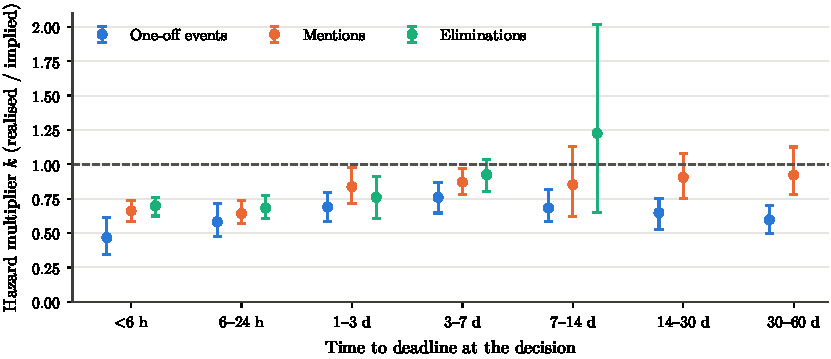
\includegraphics[width=\textwidth]{figures/fig_haz_calibration.pdf}
\caption{Hazard multiplier $k$ (realised over implied cumulative hazard) by lead and contract type,
all splits pooled, with 5th--95th percentile intervals from 200 cluster-bootstrap resamples. The
dashed line is perfect calibration. Cells with fewer than 30 observations are omitted.}
\label{haz-fig-calib}
% source: summary.json:calibration_by_kind_lead
\end{figure}

\subsubsection{Implied hazard term structures}\label{haz-res-term}

Across strips, the forward hazard curve is more often rising than flat. Of 3{,}019 daily snapshots
on 194 strips, 48\% are rising, 35\% front-loaded, 15\% flat and 2.4\% inverted, and the median ratio
of the last forward hazard to the spot hazard is 1.20 (\cref{haz-tab-term}).
% source: summary.json:term_structure_shapes
The shape differs by category in an interpretable way:
\begin{itemize}
\item Science and technology strips, mostly product-release dates, are rising in 61\% of snapshots
  with a median ratio of 2.0. The market expects a release later rather than sooner.
\item Climate strips (storm and seasonal milestones) are also rising.
\item Entertainment, sports and elections lean front-loaded (median ratios 0.70--0.89): if the
  occurrence does not come soon, it becomes less likely.
\item Politics is mixed, with a median ratio of 1.10.
\end{itemize}

Along a single contract, the implied hazard rises steeply as the deadline approaches without an event
(\cref{haz-fig-path-theta}a). Relative to its value seven days out, the median $\hbarimp$ is 1.4 times
higher at 72 hours, 2.3 times at 24 hours, 7 times at 6 hours and 33 times at one hour for politics.
Science and technology and entertainment follow nearly the same path; mentions are milder, at 10
times at one hour.
% source: summary.json:decay_paths_by_category (anchor 168 h)
A flat deterministic hazard would keep this ratio at one. Taken at face value, prices imply a hazard
concentrated near the deadline; the timing evidence below shows that realised hazards are concentrated
there too, but by much less.

\begin{table}[t]
\centering
\begin{threeparttable}
\caption{Hazard term-structure shapes and static-arbitrage frequency by category}\label{haz-tab-term}
\footnotesize
% source: summary.json:term_structure_shapes:by_category and summary.json:static_arbitrage_by_category
\setlength{\tabcolsep}{4pt}
\begin{tabular}{@{}lrrrrrrrrrr@{}}
\toprule
 & \multicolumn{6}{c}{Forward-hazard shape (daily snapshots)} & \multicolumn{4}{c}{Adjacent nested pairs (hourly)} \\
\cmidrule(lr){2-7}\cmidrule(l){8-11}
Category & Snap. & Strips & $h_{\mathrm{fwd}}/h_{\mathrm{spot}}$ & Rising & Front & Inv. & Pair-h & $p_1>p_2$ & Crossed & Exec. \\
\midrule
Politics          & 1{,}631 & 102 & 1.10 & 0.44 & 0.35 & 0.024 & 63{,}520 & 0.022 & 0.0016 & 0.0008 \\
Science \& tech.  &    783 &  38 & 2.02 & 0.61 & 0.29 & 0.022 & 32{,}955 & 0.033 & 0.0012 & 0.0007 \\
Entertainment     &    400 &  22 & 0.89 & 0.41 & 0.45 & 0.022 & 15{,}108 & 0.060 & 0.0017 & 0.0012 \\
Sports            &    126 &  17 & 0.70 & 0.43 & 0.48 & 0.048 & 14{,}173 & 0.044 & 0.0018 & 0.0011 \\
Elections         &     46 &   9 & 0.89 & 0.39 & 0.46 & 0.022 &  2{,}196 & 0.010 & 0.0005 & 0.0005 \\
Climate \& weather &    33 &   6 & 1.74 & 0.70 & 0.09 & 0.000 &  2{,}467 & 0.149 & 0.0004 & 0.0004 \\
\midrule
All               & 3{,}019 & 194 & 1.20 & 0.48 & 0.35 & 0.024 & 130{,}419 & 0.034 & & \\
\bottomrule
\end{tabular}
\begin{tablenotes}\footnotesize
\item Left: one snapshot per strip and day (16:00 UTC candle, spread at most 10\textcent), legs open,
windows started and nested. $h_{\mathrm{fwd}}/h_{\mathrm{spot}}$ is the median ratio of the last
forward hazard to the spot hazard to the first deadline. Rising: ratio above 1.25; Front: below 0.8;
Inv.: some forward hazard negative; the remaining share is flat. Right: adjacent nested legs quoted in
the same hourly candle. $p_1>p_2$: the earlier deadline's mid exceeds the later one's. Crossed: the
earlier bid exceeds the later ask. Exec.: the crossing survives the taker fee on both legs. Shares of
pair-hours; all splits pooled.
\end{tablenotes}
\end{threeparttable}
\end{table}

\subsubsection{Theta: prices decay too slowly near the deadline}\label{haz-res-theta}

Conditional on no event, prices fall more slowly than the flat-hazard theta at every lead
(\cref{haz-tab-theta}). The realised no-event change is 28--69\% of the model change, and the gap is
significant everywhere ($t$ between 3.6 and 11.5). Jumps are also rarer than the implied hazard
predicts: 18 against 74 expected in the last six hours, and 40 against 98 at 6--24 hours. The two
effects net out to a near-zero martingale drift at most leads. The exception is the last six hours,
where prices fall by 0.86\cents{} per grid step on average ($t=-7.2$), and marginally the 14--30 day
leads ($-1.3$\cents, $t=-2.1$).
% source: summary.json:theta (group core)
Read together, slow decay and rare jumps mean that the price path is close to a martingale away from
the deadline but not in the final hours. In those hours the excess is not removed by decay and is
paid off only at settlement.

\begin{table}[t]
\centering
\begin{threeparttable}
\caption{Theta, jumps and martingale drift over the next grid step (events, mentions and counts)}\label{haz-tab-theta}
\footnotesize
% source: data/research/pm_hazard/summary.json:theta (group = core)
\begin{tabular}{@{}lrrrrrrrr@{}}
\toprule
 & & & \multicolumn{2}{c}{Jumps} & \multicolumn{3}{c}{No-event change (\textcent)} & \\
\cmidrule(lr){4-5}\cmidrule(lr){6-8}
Lead & $n$ (cl.) & Drift \textcent{} ($t$) & Real. & Flat & Real. & Flat & Ratio ($t$ gap) & $\sigma_{\ln\hbarimp}$ \\
\midrule
$<6$ h   & 3{,}580 (451) & $-0.86$ ($-7.18$) &  18 &  74.2 & $-1.19$ & $-1.85$ & 0.65 (10.1) & 2.23 \\
6--24 h  & 3{,}108 (355) & $-0.35$ ($-1.55$) &  40 &  98.1 & $-1.14$ & $-2.40$ & 0.48 (10.2) & 1.22 \\
1--3 d   & 2{,}771 (317) & $0.34$ ($1.12$)   &  72 & 168.9 & $-1.23$ & $-4.43$ & 0.28 (11.5) & 0.79 \\
3--7 d   & 2{,}994 (321) & $-0.31$ ($-0.58$) & 243 & 341.3 & $-4.42$ & $-6.40$ & 0.69 (3.6)  & 0.53 \\
7--14 d  & 1{,}303 (240) & $-0.28$ ($-0.59$) &  27 &  82.2 & $-1.38$ & $-3.98$ & 0.35 (5.6)  & 0.39 \\
14--30 d & 1{,}188 (238) & $-1.30$ ($-2.10$) &  65 & 126.1 & $-3.76$ & $-6.00$ & 0.63 (4.5)  & 0.27 \\
30--60 d &    792 (189) & $-0.28$ ($-0.32$) &  70 & 106.0 & $-3.83$ & $-6.38$ & 0.60 (3.6)  & 0.21 \\
\bottomrule
\end{tabular}
\begin{tablenotes}\footnotesize
\item Priced observations (spread at most 10\textcent, mid below 0.9, no event yet), all splits pooled;
the step runs to the next grid point (to $T$ at the 1-hour lead). Drift: mean price change with the
price set to 1 after a jump, $t$ clustered by event. Jumps: realised count against the flat-hazard
expectation $\sum(1-e^{-\hbarimp\Delta})$. No-event change: mean realised mid change against the
flat-hazard theta $(1-p)(1-e^{\hbarimp\Delta})$. Ratio: realised over model, with the clustered $t$ of
their difference. $\sigma_{\ln\hbarimp}$: standard deviation of $\Delta\ln\hbarimp/\sqrt{\Delta}$ per
square-root day on no-jump steps. Conditioning on ``no event'' uses the event-time upper bound and is
descriptive.
\end{tablenotes}
\end{threeparttable}
\end{table}

\Cref{haz-fig-path-theta}b follows the 15--50\cents{} cohort from seven days out. With no event, the
mean price is still 41\% of its starting level 24 hours before the deadline (the flat model gives
16\%), 28\% at six hours (model 4\%) and 15\% one hour before (model 0.7\%). In levels this is
10.4\cents{} against 4.2\cents{} at 24 hours and 3.2\cents{} against 0.2\cents{} at one hour.
% source: summary.json:decay_paths (anchor 168, group core, p0_b 15-50)
Longshots starting below 15\cents{} (mean 5.6--6.2\cents) settle on a plateau of 1.4--2.1\cents{}
inside the last day, against model values of 0.03--0.9\cents. This plateau is largely the tick floor.
% source: summary.json:decay_paths (p0_b longshot<15)
Eliminations show the scheduled-event version of the same picture: no-event decay is only 12--31\%
of flat theta beyond six hours, because the price should not decay until the episode airs.
% source: summary.json:theta (group elimination)

\begin{figure}[t]
\centering
\begin{subfigure}[t]{0.49\textwidth}
\centering
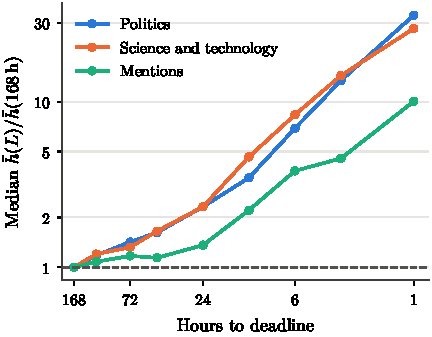
\includegraphics[width=\textwidth]{figures/fig_haz_hazard_path.pdf}
\caption{Median implied hazard relative to 168 h}
\end{subfigure}\hfill
\begin{subfigure}[t]{0.49\textwidth}
\centering
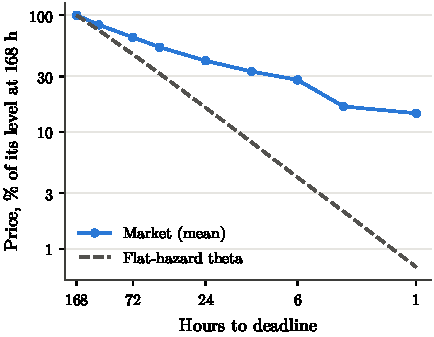
\includegraphics[width=\textwidth]{figures/fig_haz_theta.pdf}
\caption{Theta path, 15--50\textcent{} cohort}
\end{subfigure}
\caption{Implied hazard and price paths of deadline contracts with no event yet, anchored seven days
(168 h) before the deadline. (a)~Median of $\hbarimp(L)/\hbarimp(168\,\mathrm{h})$ for the three
largest categories; a flat deterministic hazard gives one (dashed). (b)~Mean price relative to its
anchor value for contracts priced 15--50\textcent{} at the anchor, against the flat-hazard theta path
$[1-(1-p_A)^{\tau_L/\tau_A}]/p_A$ (dashed). Both axes are logarithmic. Conditioning on no event uses
the event-time upper bound and is descriptive.}
\label{haz-fig-path-theta}
% source: summary.json:decay_paths_by_category; summary.json:decay_paths (core, 15-50, anchor 168)
\end{figure}

\subsubsection{When do deadline events happen?}\label{haz-res-timing}

Resolutions arrive later in the window than the flat implied hazard predicts
(\cref{haz-fig-timing-var}a). For the 807 event, mention and count contracts that resolved YES (238
clusters), the mean probability integral transform is 0.61 ($t=7.7$; Kolmogorov--Smirnov distance
0.16). Of these resolutions, 15.7\% fall in the last tenth of the window against 6.4\% under the flat
hazard, and 20\% in the final day.
% source: summary.json:event_timing:all_core
One-off events are the most back-loaded (mean PIT 0.65, $t=8.3$; 19.7\% in the last tenth). Mentions
follow at 0.60 ($t=4.6$), while counts are consistent with a flat hazard (0.52, $t=0.35$). Eliminations
are a scheduled reveal: their PIT is 0.95 and 84\% of resolutions fall in the last tenth.
% source: summary.json:event_timing:by_kind

This evidence and the calibration results fit together. Realised hazards do rise towards the
deadline, which is why a flat hazard misplaces events. But the market's implied hazard rises much
faster (\cref{haz-fig-path-theta}a). In the final six hours, the realised number of resolutions is a
quarter of what the prevailing implied hazards predict (18 against 74, \cref{haz-tab-theta}). The net
result is a deadline premium concentrated in the final day.

\begin{figure}[t]
\centering
\begin{subfigure}[t]{0.49\textwidth}
\centering
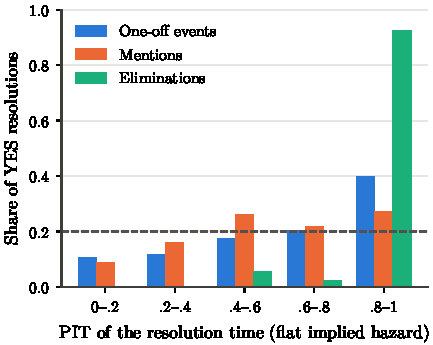
\includegraphics[width=\textwidth]{figures/fig_haz_timing.pdf}
\caption{Event timing}
\end{subfigure}\hfill
\begin{subfigure}[t]{0.49\textwidth}
\centering
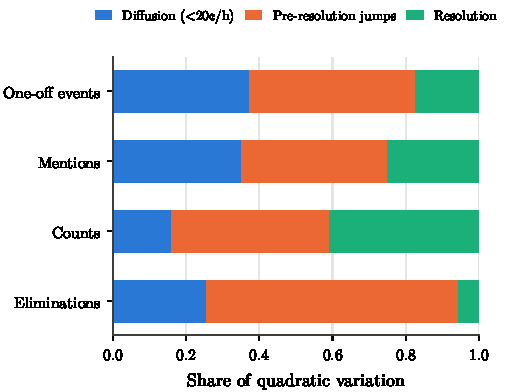
\includegraphics[width=\textwidth]{figures/fig_haz_variance.pdf}
\caption{Variance decomposition}
\end{subfigure}
\caption{(a)~Distribution of the probability integral transform of YES resolution times under the
flat hazard implied by the first priced pre-event quote; uniform (dashed) if the implied hazard shape
were right. (b)~Shares of the quadratic variation of the hourly mid up to settlement: diffusion
(hourly changes below 20\textcent), jumps of at least 20\textcent{} before resolution, and the
resolution step (the YES jump plus the NO deadline step).}
\label{haz-fig-timing-var}
% source: summary.json:event_timing:by_kind; summary.json:jump_diffusion_qv
\end{figure}

\subsubsection{Jumps, diffusion and the implied-hazard process}\label{haz-res-jumps}

Most price variance before resolution is news, not the resolution itself
(\cref{haz-fig-timing-var}b). For the 4{,}032 event, mention and count contracts with enough hourly
quotes, hourly changes below 20\cents{} account for 34\% of quadratic variation, and jumps of at
least 20\cents{} before resolution (about 0.5 per contract) for 42\%. The YES resolution jump accounts
for 23\%, and the NO deadline step for 0.8\%. Prices of contracts that resolve YES stand at 84\cents{}
on average two hours before the event-time bound, so the final jump averages 16\cents. The total is
1.19 times $\sum p_0(1-p_0)$, close to the martingale identity, with the excess consistent with
bid-ask bounce. Among events, mentions and counts, the YES resolution share is smallest for one-off events (16\%)
and largest for counts (37\%).
Eliminations are dominated by pre-resolution jumps (69\%), as episodes reveal information in large
steps.
% source: summary.json:jump_diffusion_qv

The implied hazard itself diffuses, with a volatility that rises towards the deadline. The standard
deviation of $\Delta\ln\hbarimp$ is 0.21--0.39 per square-root day beyond a week and 2.2 within six
hours (\cref{haz-tab-theta}). A CIR fit (\cref{haz-eq-cir}) is rejected as a description of
$\hbarimp$: the estimated mean reversion is negative at every horizon, $\kappa=-0.05$ per day beyond
three days and $-2.0$ within three days. The implied average hazard drifts upward towards the
deadline instead of reverting (\cref{haz-tab-cir}). A Cox model for these contracts therefore needs a
deterministic deadline-shaped component in the intensity, with diffusion around it of roughly 0.4 per
square-root day in log terms far from the deadline.
% source: summary.json:cir (group core)

\subsubsection{Static arbitrage across strips}\label{haz-res-arb}

Monotonicity violations are common at the mid but almost never executable (\cref{haz-tab-term}). Over
130{,}419 pair-hours on 898 adjacent nested pairs, the earlier deadline's mid exceeds the later one's
3.4\% of the time, but the earlier bid exceeds the later ask in only 0.04--0.18\% of pair-hours by
category. After taker fees, 108 pair-hours on 52 pairs in 36 strips remain, with a median locked-in
payoff of 0.8\cents{} per pair at unknown displayed size.
% source: summary.json:term_structure:monotonicity; summary.json:static_arbitrage_by_category
Calendar spreads show that forward segments are overpriced as well. In the \estim, the implied
conditional probability of an event between the two deadlines is 0.27 against a realised 0.21, and
buying the forward (NO on the near leg, YES on the far leg) loses 8.5\cents{} per pair ($t=-5.0$).
In the holdout it loses 7.2\cents{} ($t=-2.2$; 105 observations on 31 pairs).
% source: summary.json:term_structure:calendar

\subsubsection{Economic significance}\label{haz-res-econ}

The overpricing does not yield a robust trading rule (\cref{haz-tab-econ}). Buying NO when the
dev-fitted multiplier table shows an edge earns 19.0\cents{} per contract in-sample but $-5.3$\cents{}
($t=-0.8$; 49 trades in 13 clusters) in the holdout. A price-only calibration model does no better.
Buying NO on every quote below 50\cents{} earns 1.3\cents{} in the holdout ($t=1.65$), and 0.06\cents{}
on the first signal per contract. In a logistic blend with the mid, the hazard model's holdout
coefficient is 0.006 ($t=0.04$): out of sample it adds no information to the price.
% source: summary.json:economic

\subsubsection{Limitations}\label{haz-res-limits}
Several limitations qualify these results:
\begin{itemize}
\item The holdout is short: 2{,}076 priced observations, with at most 66 event clusters per lead cell.
% source: summary.json:universe:split_rows; summary.json:calibration_by_split
\item The event time is an upper bound. It makes resolutions look slightly late, biasing the timing
  PIT towards back-loading by an amount that is small relative to windows of days or weeks.
\item The one-cent tick floors longshot prices and explains much of their stickiness near the
  deadline.
\item History before 15 August 2026 comes from series chosen by title keyword. The choice does not
  depend on outcomes, but it can miss one-off series with other titles.
\item Strip nesting relies on the issuance order of legs.
\item The CIR fit uses an average rather than a spot intensity.
\end{itemize}
